\documentclass[a4paper]{report}

\usepackage[utf8]{inputenc}
\usepackage[russian]{babel}
\usepackage{amsmath}
\usepackage{dsfont}
\usepackage{amsfonts}
\usepackage{verbatim}
\usepackage{atbegshi}
\usepackage{tikz}
\usepackage{graphicx}
\usepackage{float}
\usepackage[affil-it]{authblk}
\usetikzlibrary{arrows}

\tikzstyle{int}=[draw, fill=blue!20, minimum size=2em]
\tikzstyle{init} = [pin edge={to-,thin,black}]

\title{Вариационные Автоэнкодеры с полимодальнымы латентными переменными.}

\author{Мазур Д. В.%
}
\affil{Школа №1505 "Преображенская"}

\author{Маргаритов В. С.%
}
\affil{Консультант}

\date{\today}

\begin{document}

\maketitle

\tableofcontents
\newpage

\chapter{Введение}
Одной из задач машинного обучения является генеративное моделирование - задача ``выучивания'' заданного вероятностного распределения. Генеративное
моделирование может решать как задачу аппроксимации зависимости какой-либо переменной от другой ($p(x \mid y)$), так и задачу выучивания распределения
одной переменной $p(x)$. Последняя задача успешно решается вариционными автоэнкдерами. Тем не менее метод имеет некоторые фундаментальные недостатки,
которые приводят к низкой вариативности генерируемых данных. Например, картинки, генерируемые вариационным автоенкодером, получаются размытыми, так
как таким образом больше похожи на наиболее вероятный элемент выборки, а значит сами имеют большую вероятность. В этой работе мы собираемся решить
эту проблему методом, описынным в параграфе \ref{solution}.


\chapter{Обучение нейронных сетей}
Для базового понимания автоенкодеров не требуется понимание принципа работы нейронных сетей, по этой причине объяснение устройства нейронных сетей было решено опустить 
и уделить больше внимания принципу их обучения. Для интересующихся, литература на тему нейронных сетей будет приложина в библиографии.

Для простоты устройсто нейронной сети можно редуцировать до некоторой функции, имеющей параметы $W$, принимающей значения $X$ и выдающей значения $\widehat{X}$. 
Физический смысл $X$ - данные, подаваемые на вход сети, $\widehat{X}$ - выход нейронной сети. Каждому элементу $x \in X$ соответсвует элемент $y \in Y$, и задачей обучения
нейронной сети является подобрать параметы $W$ нейронной сети так, чтобы они минимально или не отличались от $Y$. Также можно сформулировать задачу следущим образом:

$$d(f(x_n), y_n) \rightarrow \text{min}$$

Также, можно поставить задачу как поиск оптмальных параметров $W$:

$$\underset{W}{\textbf{argmin }} d(f(x_n), y_n)$$ 

Где $f(x)$ - нейронная сеть, а $d(x, y)$ определенная нами функция расстояния (отличия) между выходом нейронной сети и настоящим ответом, называемая функцией потерь.
Важно понимать следующие свойства функций $f(x)$ и $d(x, y)$, они обе дифференцируемые и определены на всех $X$, а это значит, что мы к параметрам нейронной сети $W$ можем
применять любые методы оптимизации функций, например, градиентный метод.

\section{Градиентный метод}
Градиентый метод является методом решения задач вида $\underset{a \in \mathds{R}^n}{\textbf{min }} g(x)$. Алгоритм градиентного метода начинается с выбора
параметоров $a$, это может делать как и из какого либо представления того какими примерно эти парамерты должны быть, так и случайным образом. Далее
идет так называемый "шаг" градиентного метода. Из параметров $a$ вычитаеся значение градента функции $g(a)$ в точке текущего значения $a$:

$$ a_{n + 1} = a_n - \nabla g(a_n)$$

Чтобы не "перескочить" через минимум функции во время итерации метода, градиент $\nabla f(x)$ обычно умножается на какую-то константу $\alpha$:

$$ a_{n + 1} = a_n - \alpha \nabla g(a_n)$$

\subsection{Градиентный метод в обучении нейронных сетей}
Теперь о том как градиентный метод может применяться в обучении нейронных сетей.

Функцию потерь нейронной сети $d(f(x_n), y_n)$ можно записать в виде, $d(f(x_n, W), y_n)$, до этого, для простоты, записи парамерты нейронной сети $W$ не записывались
как аргумент, хотя, очевидно, им являются. Поясню, что X и Y являются константными значениями, так как являются выборкой наших
данных и известны нам заранее. Таким образом, единственный аргумент, который мы можем изменять, минимизируя функцию потерь - $W$.

На практике, оптимизировать функцию потерь градиентным спуском "в лоб" не получится. У этого есть несколько причин, одна из главных - риск переобучения
модели (ситуация при которой модель показывает идеальных результат на обучающей выборке, но плохой на валидации). Но помимо этого, выборка данных
чаще всего слишком велика и не помещается в память компьютера, по этой причине на каждой итерации градиентного метода выбирается случайная подвыборка
тренировочных данных и над ней совершается шаг граиентого метода. Данный метод называется стохастическим градиентным спуском.

\chapter{Вариационные автоэнкодеры}

\section{Модели с латентными переменными}

Предположим, что мы хотим моделировать какую-либо систему с помощью вероятностого распределения её состояний $p(\mathbf{x})$, где
$\mathbf{x} \in \mathcal{R}^D$. Такая система может быть достаточно сложной и мы можем не знать явный вид $p(\mathbf{x})$. Для решения этой проблемы
можем ввести новую переменную $\mathbf{z} \in \mathcal{R}^d$, которая описывает состояния $\mathbf{x}$, например если $\mathbf{x}$ - картинки котиков, то
$\mathbf{z}$ может описывать их цвет, породу и положение на картинке. Подобные переменные называются ``латентными''.
Также новая переменная позволяет нам выразить $p(\mathbf{x})$ как:

\begin{align*}
    p(\mathbf{x}) = \int p(\mathbf{x} \mid \mathbf{z}) p(\mathbf{z}) ~d\mathbf{z}
    \tag{1}
\end{align*}

Имея подобную систему нам бы хотелось знать плотность распределения самих латентных переменных $\mathbf{z}$, при том, что мы знаем соответсвующий
им $\mathbf{x}$. Если быть точнее, то мы хотим знать апостериорное распределение $p(\mathbf{z} \mid \mathbf{x})$. Но зависимость между $\mathbf{x}$ и
$\mathbf{x}$ может быть крайне нелинейной, а размерности $D$ и $d$ достаточно большими, а так как и частное распределение $p(\mathbf{x})$ и апостериорное
распределение $p(\mathbf{z} \mid \mathbf{x})$ требуют вычисления интеграла, они не поддаются вычислению.

\begin{comment}
    про трудность решения методом монте-карло
\end{comment}

Но решить эту проблему можно с помощью параметрического распределения, параметры которого задаются нейронной сетью с параметрами $\theta \in \Theta$.
Таким образом мы можем выучить оптимальные параметры с помощью метода максимального правдоподобия:

\begin{align*}
   \theta^* = \arg \max_{\theta \in \Theta} p_\theta(\mathbf{x}) 
   \tag{2}
\end{align*}

Но мы всё ещё не можем максимизировать выражение (1), значение которого мы не можем вычислить. Для решения этой проблемы мы можем применить метод
выборки по значимости (importance sampling). Когда нам нужно оценить величину из какого либо первичного вероятностого распределения, выборка по
значимости позволяет нам выбирать величины из другого (смещённого) распределения и взвешивать новые велечины через функцию плотности вероятности 
первичного распределения. В нашем случае это нам поможет, так как мы не можем напрямую выбирать переменные из $p(\mathbf{z})$. Пусть $q_\phi(\mathbf{z} \mid \mathbf{x})$ 
будет смещённым распределением, заданным нейронной сетью с параметрами $\phi \in \Phi$. Теперь мы можем записать $p(\mathbf{x})$ как:

\begin{gather*}
    p(\mathbf{x}) = \int p(\mathbf{z})p_\theta(\mathbf{x} \mid \mathbf{x})~d\mathbf{z} =\\
        \mathbb{E}_{p(\mathbf{z})} \left[p_{\theta}(\mathbf{x} \mid \mathbf{z})\right] = 
        \mathbb{E}_{p(\mathbf{z})} \left[\frac{q_\phi(\mathbf{z} \mid \mathbf{x})}{q_\phi(\mathbf{z} \mid \mathbf{x})}p_{\theta}(\mathbf{x} \mid \mathbf{z})\right] =
        \mathbb{E}_{q_\phi(\mathbf{z} \mid \mathbf{x})} \left[\frac{p(\mathbf{x} \mid \mathbf{z})p(\mathbf{z})}{q_\phi(\mathbf{z} \mid \mathbf{x})}\right]
    \tag{3}
\end{gather*}

В методе выборки по значимости оптимальные переменные пропорциональны функции плотности первичного распределения, в нашем случае это распределение
$p_\theta(\mathbf{x} \mid \mathbf{z})$, пременив теорему Байеса мы получим $p_\theta(\mathbf{x} \mid \mathbf{z}) 
= \frac{p_\theta(\mathbf{z} \mid \mathbf{x}) p_\theta(\mathbf{x})}{p_\theta(\mathbf{z})}$. Как мы можем наблюдать, оптимальные переменные пропорциональны
апостериорному распределению $p_\theta(\mathbf{z} \mid \mathbf{x})$, которое, конечно, невычислимо.

\section{Вариационные автоэнкодеры}
К счастью, мы можем решить эту проблему. Пытаясь аппроксимировать апосетриорнoе распределение выученным смещённым распределением\\ 
($q_\phi(\mathbf{z} \mid \mathbf{x})$), мы можем неплохо аппроксимировать $p_\theta(\mathbf{x})$. Подобная система похожа на модель, называемой
автоенкодером, в которой есть некоторый энкододер $q_\phi(\mathbf{z} \mid \mathbf{x})$ и декодер $p_\theta(\mathbf{x} \mid \mathbf{z})$.

Разберём подробнее, что делают энкододер и декодер. Декодер - генеративная модель $p_\theta(\mathbf{x}, \mathbf{z})$, состоящая из самого декодера
$p_\theta(\mathbf{x} \mid \mathbf{z})$ и приорного распределения латентных переменных $p(\mathbf{z})$. По-сути декодер преобразует латентные переменные
$\mathbf{z}$ в моделируемые переменные $\mathbf{x}$. Енкодер $q_\phi(\mathbf{z} \mid \mathbf{x})$ осуществляет обратную операцию преобразования моделируемых
переменных $\mathbf{x}$ в латентные переменные $\mathbf{z}$.

Так как и энкододер и декодер в нашей системе заданы как нейронные сети, мы можем обучать их, оптимизируя параметры градиентным методом, а
значит нам нужна функция потерь. В данном случае мы хотим сделать распределения $p_\theta(\mathbf{z} \mid \mathbf{x})$ и $q_\phi(\mathbf{z} \mid \mathbf{x})$
максимально похожими на друг-друга. Для этого мы можем минимизировать какую-либо функцию расстояния между ними, возьмём, например, девергенцию
Кульбака-Лейблера:

\begin{gather*}
    KL(q_\phi(\mathbf{z} \mid \mathbf{x}) || p_\theta(\mathbf{z} \mid \mathbf{x})) 
    = \int q_\phi(\mathbf{z} \mid \mathbf{x}) \frac{q_\phi(\mathbf{z} \mid \mathbf{x})}{p_\theta(\mathbf{z} \mid \mathbf{x})}~d\mathbf{x} =\\
    \mathbb{E}_{q_\theta(\mathbf{z} \mid \mathbf{x})} \left[\log q_\phi(\mathbf{z} \mid \mathbf{x}) - p_\theta(\mathbf{z} \mid \mathbf{x})\right]
\end{gather*}

Разумеется, мы не можем напрямую посчитать это ``расстояние'' по причине того, что нам неизвесты оба апостериорных распределения, \\
но решить эту проблему можно решая двойственную задачу, называемой Evidence Lower Bound (ELBo):

\begin{align*}
     KL&(q_\phi(\mathbf{z} \mid \mathbf{x}) || p_\theta(\mathbf{z} \mid \mathbf{x})) \\
    &= \int q_\phi(\mathbf{z} \mid \mathbf{x}) \frac{q_\phi(\mathbf{z} \mid \mathbf{x})}{p_\theta(\mathbf{z} \mid \mathbf{x})}~d\mathbf{x}\\
    &= \mathbb{E}_{q_\theta(\mathbf{z} \mid \mathbf{x})} \left[\frac{q_\phi(\mathbf{z} \mid \mathbf{x})}{p_\theta(\mathbf{z} \mid \mathbf{x})}\right]\\
    &= \mathbb{E}_{q_\theta(\mathbf{z} \mid \mathbf{x})} \left[\log q_\phi(\mathbf{z} \mid \mathbf{x}) - \log p_\theta(\mathbf{z} \mid \mathbf{x})\right]\\
    &= \mathbb{E}_{q_\theta(\mathbf{z} \mid \mathbf{x})} \left[\log q_\phi(\mathbf{z} \mid \mathbf{x}) - \log p(\mathbf{x}, \mathbf{z})\right] + \log p_\theta(\mathbf{x})\\
    &= \mathcal{L}(\mathbf{x}, \theta, \phi) + \log p_\theta(\mathbf{x})
\end{align*}

На четвёртой строчке мы раскрываем логарифм, на пятой мы примениям теорему Байеса и пользуемся тем, что $p(\mathbf{x})$ независим от $\mathbf{z}$. Данное
выражение мы можем переписать следущим образом:

\begin{align*}
  \log p_\theta(\mathbf{x}) = \mathcal{L} (\mathbf{x}; \theta, \phi) + KL \left( q_\phi (\mathbf{z} \mid \mathbf{x}) || p_\theta(\mathbf{z} \mid \mathbf{x}) \right)
\end{align*}

\begin{align*}
  \mathcal{L} (\mathbf{x}; \theta, \phi) = \mathbb{E}_{q_\phi (\mathbf{z} \mid \mathbf{x})}
    \left[
      \log \frac{
        p_\theta (\mathbf{x}, \mathbf{z})
      }{
        q_\phi (\mathbf{z} \mid \mathbf{x})
      }
    \right].
\end{align*}

Мы можем приближённо вычислить ELBo, используя один элемент из нашего смещённого распределения $q_\phi(\mathbf{z} \mid \mathbf{x})$:
\begin{align*}
   \mathcal{L} (\mathbf{x}; \theta, \phi) \approx  \log \frac{
      p_\theta (\mathbf{x}, \mathbf{z})
    }{
      q_\phi (\mathbf{z} \mid \mathbf{x})
    }, \qquad \mathbf{z} \sim q_\phi (\mathbf{z} \mid \mathbf{x}). 
\end{align*}

Имея функцию потерь (ELBo) мы можем найти оптмальые параметры $\phi$ и $\theta$ с помощью градиентного спуска:
\begin{align*}
  \phi^\star,~\theta^\star = \arg \max_{\phi \in \Phi,~\theta \in \Theta}
  \mathcal{L} (\mathbf{x}; \theta, \phi).  
\end{align*}

Для большей понятности архитектура автоенкодера изображена на рисунке:
\begin{figure}[H]
  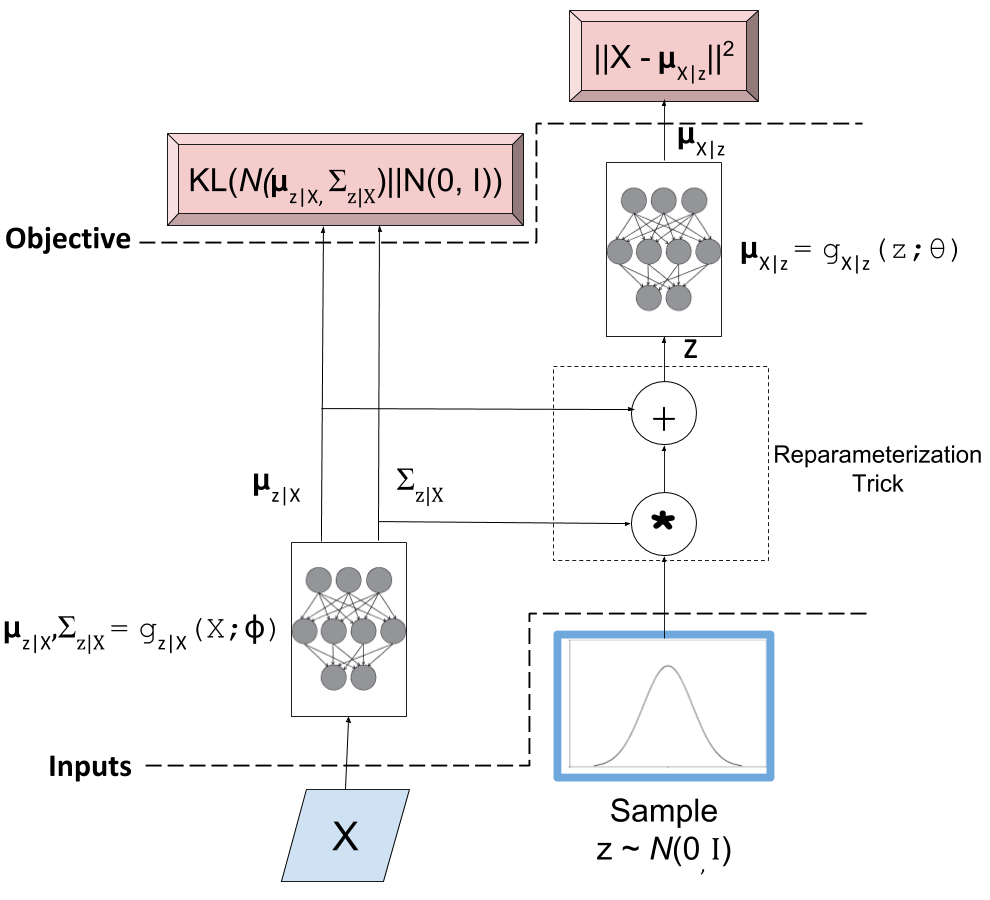
\includegraphics[width=\linewidth]{vae.png}
  \caption{Архитектура Вариационного автоенкодера}
  \label{fig:vae}
\end{figure}

\chapter{Практическая часть}

\section{Недостатки вариационных автоэнкдеров}

При построении декодера нашей модели мы предполагаем, что $\mathbf{z}$ распределены нормально, то есть $p(\mathbf{z})$ имеет плотность нормального
распределения. Но в большинсве случаев это распределение имеет более сложную форму, часто полимодальное. По этой причине распределения изображений,
моделируемые вариационными автоэнкдерами часто получаются размытими.

Решением этой проблемы могло бы быть минимизировать девергенцию Кульбака-Лейблера не между нашей моделью и нормальным распределением, а, например,
смесью нормальных распределений. Проблема в этом случае заключается в том, что параметры приближаемого распределения выбираются произволно, а посему
будут требовать долгой подборки оптимальных параметров.

\section{Решение} \label{solution}

Решить эту проблему можно дав нейронной сети возможность самостоятельно выбирать параметры приближаемого распределения. Осуществить это можно
следующим образом: вместо того, чтобы генерировать вектор латентных переменных $\mathbf{z}$ размером $d$, генерировать матрицу размерности $d \times N$, где
$N$ - число гауссиан из которых нейронная сеть может выбирать. Выбор параметров гауссины осуществляется с помощью генерации onehot-матрицы D размерности 
$d \times N$. Onehot-матрица - это матрица, которая имеет одну еденицу на каждой строчке, а остальные компоненты равны нулю. После этого матрица поэлементно умножается
на параметры распределений, заданных $z$. После чего строчки полученной матрицы суммируются, получая вектор размера $d$. Подробный алгоритм получения
новых $z$ показан на русунке \ref{fig:musigma}

\begin{figure}[H]
  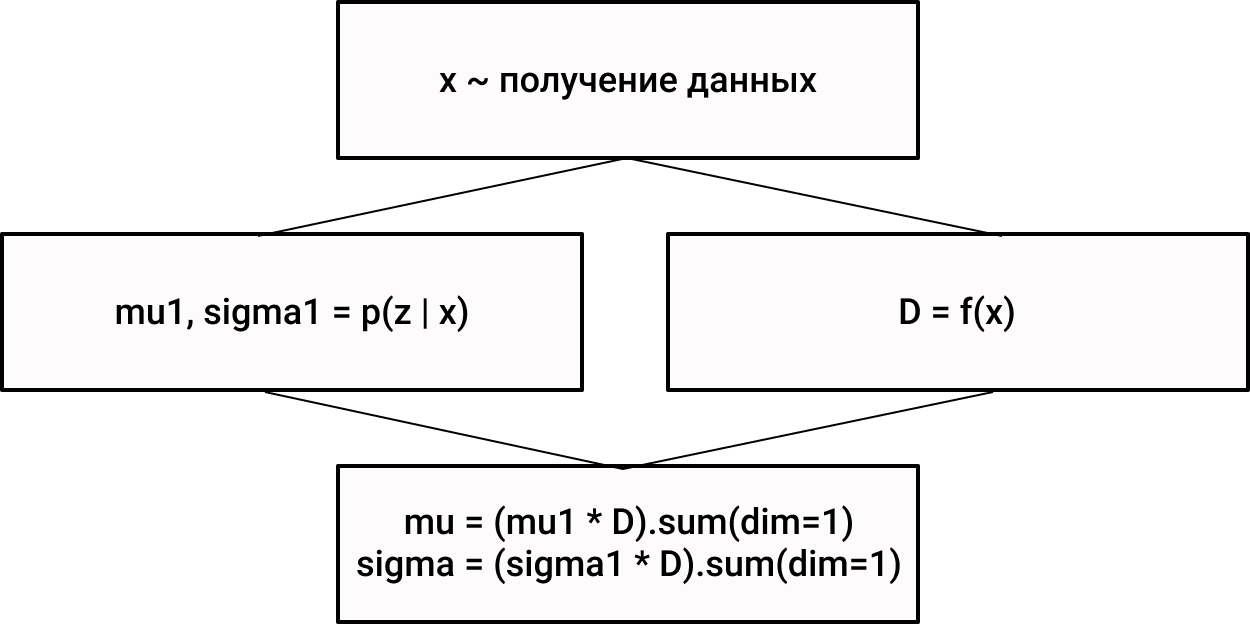
\includegraphics[width=\linewidth]{block-diagram.png}
  \caption{Блок схема получаения $\mu$ и $\sigma$}
  \label{fig:musigma}
\end{figure}

\section{Методы}
Для написания нейронных сетей использовалась библиотека pytorch для языка python. Код писался в среде vscode для модулей нейронной\\ 
сети и jupyter для постановки экспериментов. Код доступен на сайте\\
https://github.com/deniskamazur.

\section{Результаты}

После экспериментов выяснилось, что предложенный алоритм не справляется с задачей сильно лучше классического вариационного автоенкодера.
Для сравнения моделей использовалась метрика SNR (signal-noise-ratio), которая показала почти одинаковое значение для обоих методов $\approx 0.8$ 
Причина этого лежит в том, что на ранних стадиях обучения модели, когда иметь большую вариативность в $\mathbf{z}$ для модели невыгодно. 
По этой причине нейросеть сильно завышает уверенность в одной из компонент смеси нормальных распределений. П
одобная проблема называется ``model collapse''.

Решением этой проблемы может быть штрафовать нейронную сеть сильную уверенность в выборе гауссианы, например с помощью регуляризации высов.

\section{Дальнейшкая работа}

В дальнейшем планируется решить проблему коллапсирующих мод для нашего алгоритма. В планах опробовать дла подхода к решению проблемы:
регуляризация весов и метод ``hierarchical priors'', который показыват хорошие результаты в решении проблем коллапсирующих категориальных распредений.

\newpage
\begin{thebibliography}{9}

\bibitem{edwardlib}
Edward 
[\textit{KL($q || p$) Minimization}]

\bibitem{isampling}
Brian Keng
[\textit{Importance Sampling and Estimating Marginal Likelihood in Variational Autoencoders}] 

\bibitem{vae}
Diederik P Kingma, Max Welling
[\textit{Auto-Encoding Variational Bayes}] 

\bibitem{kiosorek}
Adam Kosiorek
[\textit{Auto-Encoding Variational Bayes}] 

\bibitem{random}
[\textit{Probability, Mathematical Statistics, Stochastic Processes}] 

\bibitem{stanford}
Stanford University
[\textit{Stanford Statistics }] 



\end{thebibliography}
\end{document}